\chapter{Finite State Machines}\label{ch:fsm}

\begin{objectives}
After studying this chapter you will be able to:
\begin{itemize}
  \item describe a finite state machine (FSM) by its next-state logic, state memory and output logic, and distinguish the Moore from the Mealy model;
  \item analyse an FSM from its circuit and synthesise one from a word description, using state diagrams, state tables and K-maps;
  \item apply the design procedure to counters, controllers and one-shot circuits;
  \item write FSMs in VHDL with the two-process method and the \code{numeric_std} type conversions;
  \item compare Moore and Mealy implementations of the same function, in the number of states, the output timing and the risk of glitches; and
  \item state the clock-period constraint of a synchronous FSM and choose a state encoding.
\end{itemize}
\end{objectives}

\section{Finite State Machines}\label{sec:fsm-recall}
A \term{finite state machine} (FSM) is a computational model with a finite number of \emph{states}; it moves between states according to its inputs and its present state, and produces outputs. Every synchronous sequential circuit of \cref{ch:latches} is an FSM, and an FSM is the standard way to describe a controller. It has three parts (\cref{fig:fsm-general}):
\begin{enumerate}
  \item \textbf{next-state logic}, a combinational circuit that computes the next state from the present state and the inputs;
  \item \textbf{state memory}, the flip-flops (the \term{state register}) that hold the present state and are updated at each clock edge; and
  \item \textbf{output logic}, a combinational circuit that generates the outputs.
\end{enumerate}

\figside{461.1pt}{lect_8_fsm_general_block_diagram}{General structure of an FSM: next-state logic, state register and output logic.}{fig:fsm-general}

\section{Moore and Mealy Machines}\label{sec:models}
The two FSM models differ in their output logic (\cref{fig:mealy-moore}).
\begin{itemize}
  \item \textbf{Moore machine}: $\mathrm{output}=f(\mathrm{present\ state})$. Outputs change synchronously with the state, are stable for the whole clock period and are glitch-free. The output logic is simple, but the machine often needs more states.
  \item \textbf{Mealy machine}: $\mathrm{output}=f(\mathrm{present\ state},\mathrm{inputs})$. Outputs can change as soon as the inputs change, which gives a faster response and often \emph{fewer states}, but the output can also show glitches and is not synchronised with the clock.
\end{itemize}

\figw{376.1pt}{lect_8_mealy_moore_block}{Block diagrams of the Moore and Mealy models; the only difference is whether the inputs feed the output logic.}{fig:mealy-moore}

\section{Analysis of an FSM}\label{sec:fsm-analysis}
\termx{Analysis}{analysis} determines the behaviour of a given circuit. The steps are those of \cref{sec:seq-analysis}: (1)~determine the flip-flop input equations and output equations; (2)~construct the state table; (3)~draw the state diagram, with states as nodes and transitions as arrows labelled \texttt{input/output}. Examples with D, JK and T flip-flops were given in \cref{ch:latches}; here is one with two inputs.

\begin{example}{Analysis of a one-flip-flop machine}{fsm-an}
The circuit of \cref{fig:fsm-an} has one D flip-flop $A$, two inputs $x$, $y$ and an output $z$.

\textbf{Equations.} $D_A=A\xor x\xor y$ and $z=Ax$. Since $A^+=D_A$, the state table is \cref{tab:fsm-an}. For example, in state $A=1$ with $x=1,y=0$, $A^+=1\xor1\xor0=0$ and $z=1$.

\textbf{Diagram.} The machine has two states. The output depends on the input $x$, so it is a Mealy machine (\cref{fig:fsm-an-state}).
\end{example}

\begin{table}[htbp]
\centering
\caption{State table of \cref{ex:fsm-an}.}
\label{tab:fsm-an}
\begin{tabular}{c|cc|c|c}
\toprule PS $A$ & $x$ & $y$ & NS $A^+=A\xor x\xor y$ & $z=Ax$\\ \midrule
0&0&0&0&0\\0&0&1&1&0\\0&1&0&1&0\\0&1&1&0&0\\
1&0&0&1&0\\1&0&1&0&0\\1&1&0&0&1\\1&1&1&1&1\\ \bottomrule
\end{tabular}
\end{table}

\begin{figure}[htbp]
\centering
\begin{subfigure}[b]{264.3pt}\centering
  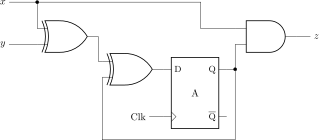
\includegraphics[width=262.3pt]{lect_8_analysis_example_fsm}\caption{circuit}\label{fig:fsm-an}
\end{subfigure}
\\[6pt]
\begin{subfigure}[b]{188.1pt}\centering
  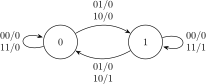
\includegraphics[width=186.1pt]{lect_8_analysis_example_state_diagram}\caption{state diagram}\label{fig:fsm-an-state}
\end{subfigure}
\caption{The circuit analysed in \cref{ex:fsm-an}.}
\end{figure}

\section{Synthesis of an FSM}\label{sec:fsm-synth}
\termx{Synthesis}{synthesis} creates a circuit from a description of behaviour.
\begin{enumerate}
  \item \textbf{Understand the specification}: inputs, outputs, initial state.
  \item Create the \textbf{state diagram}.
  \item Create the \textbf{state table}.
  \item (Optional) \textbf{state minimisation}: merge equivalent states.
  \item \textbf{State assignment}: assign binary codes to states.
  \item Choose the \textbf{flip-flop type} (D, JK, T).
  \item Derive the \textbf{logic equations} for the flip-flop inputs and outputs with K-maps.
  \item Draw the \textbf{logic diagram} and, in a modern flow, write the VHDL.
\end{enumerate}

\paragraph{State encoding.} A machine with $N$ states needs at least $\lceil\log_2N\rceil$ flip-flops. \emph{Binary} encoding uses this minimum, but the next-state logic can be complex. \emph{Gray} encoding gives adjacent states that differ in one bit, which suits counters and reduces glitches. \emph{One-hot} encoding uses $N$ flip-flops, exactly one of which is 1 in each state; it needs more flip-flops but simpler and faster logic, and is popular in FPGAs, which are rich in flip-flops. In VHDL an enumerated state type leaves the choice of encoding to the synthesis tool.

\section{Design Examples}\label{sec:fsm-examples}

\subsection{A 2-bit up/down counter}
\begin{example}{2-bit up/down counter}{updown}
Design a synchronous 2-bit counter that counts up when $x=1$ and down when $x=0$, using JK flip-flops.

\textbf{State table.} The states are 00, 01, 10, 11. For $x=1$: $00\to01\to10\to11\to00$; for $x=0$: $00\to11\to10\to01\to00$. The excitation table (\cref{tab:updown}) is obtained from the transitions of each flip-flop with the JK excitation table of \cref{tab:excit}.

\textbf{Equations.} All entries for $Q_0$ are 1 or X, so $J_0=K_0=1$ ($Q_0$ toggles on every clock). For $Q_1$ the K-maps (\cref{fig:updown-km}) give
\[
 J_1 = K_1 = x\odot Q_0 = \overline{x\xor Q_0}.
\]
Check: counting up ($x=1$), $Q_1$ must toggle when $Q_0=1$; counting down ($x=0$) it toggles when $Q_0=0$; in both cases $x\odot Q_0=1$. The circuit is \cref{fig:updown-circ}.
\end{example}

\begin{table}[htbp]
\centering
\small
\caption{Excitation table of the 2-bit up/down counter.}
\label{tab:updown}
\begin{tabular}{cc|c|cc|cccc}
\toprule
\multicolumn{2}{c|}{PS} & Input & \multicolumn{2}{c|}{NS} & $J_1$&$K_1$&$J_0$&$K_0$\\
$Q_1$&$Q_0$&$x$&$Q_1^+$&$Q_0^+$&&&&\\ \midrule
0&0&0&1&1&1&X&1&X\\0&0&1&0&1&0&X&1&X\\
0&1&0&0&0&0&X&X&1\\0&1&1&1&0&1&X&X&1\\
1&0&0&0&1&X&1&1&X\\1&0&1&1&1&X&0&1&X\\
1&1&0&1&0&X&0&X&1\\1&1&1&0&0&X&1&X&1\\ \bottomrule
\end{tabular}
\end{table}

\begin{figure}[htbp]
\centering
\begin{subfigure}[b]{346.6pt}\centering
  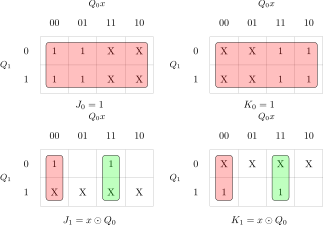
\includegraphics[width=344.6pt]{lect_8_up_down_counter_kmaps}\caption{K-maps}\label{fig:updown-km}
\end{subfigure}
\\[6pt]
\begin{subfigure}[b]{294.1pt}\centering
  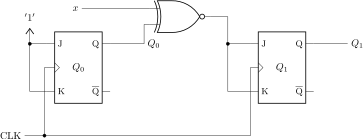
\includegraphics[width=292.1pt]{lect_8_up_down_counter_circuit}\caption{logic diagram}\label{fig:updown-circ}
\end{subfigure}
\caption{Synthesis of the 2-bit up/down counter.}
\end{figure}

\subsection{A car security system (Moore)}
\begin{example}{Car security controller}{carsec}
Design a controller with inputs $M$ (master switch), $D$ (door sensor), $V$ (vibration sensor) and output $A$ (alarm siren). The system is initially disarmed. If $M=1$ it is armed; if it is armed and a door or the vibration sensor trips, the siren sounds. Once the siren sounds it stays on until $M=0$.

\textbf{State diagram.} Two states: \emph{No\_Siren} ($Q=0$, $A=0$) and \emph{Siren} ($Q=1$, $A=1$) (\cref{fig:car-fsm}). The output depends only on the state: a Moore machine.

\textbf{State table} (\cref{tab:carsec}). The K-maps (\cref{fig:car-km}) give
\[
 Q^+ = M\,(Q + D + V),\qquad A = Q .
\]
The circuit is \cref{fig:car-circ} and \cref{lst:carsec} the VHDL.
\end{example}

\begin{table}[htbp]
\centering
\caption{State table of the car security controller.}
\label{tab:carsec}
\begin{tabular}{l|ccc|c|c}
\toprule
State $Q$ & $M$&$D$&$V$&$Q^+$&$A$\\ \midrule
0 (No\_Siren)&0&X&X&0&0\\0 (No\_Siren)&1&0&0&0&0\\0 (No\_Siren)&1&1&X&1&0\\0 (No\_Siren)&1&X&1&1&0\\
1 (Siren)&0&X&X&0&1\\1 (Siren)&1&X&X&1&1\\ \bottomrule
\end{tabular}
\end{table}

\begin{figure}[htbp]
\centering
\begin{subfigure}[b]{161.4pt}\centering
  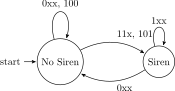
\includegraphics[width=159.4pt]{lect_8_car_security_fsm}\caption{state diagram}\label{fig:car-fsm}
\end{subfigure}
\hfill
\begin{subfigure}[b]{198.7pt}\centering
  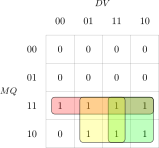
\includegraphics[width=196.7pt]{lect_8_car_security_kmaps}\caption{K-map}\label{fig:car-km}
\end{subfigure}
\\[6pt]
\begin{subfigure}[b]{262.8pt}\centering
  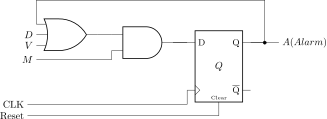
\includegraphics[width=260.8pt]{lect_8_car_security_circuit}\caption{circuit}\label{fig:car-circ}
\end{subfigure}
\caption{Car security controller.}
\end{figure}

\vhdlfile{listings/ch08_car_security.vhd}{VHDL of the car security controller: an enumerated state type, a state-register process and a combinational process (the two-process method).}{lst:carsec}

The VHDL uses an \emph{enumerated type} to give names to the states, so the designer does not have to choose binary codes by hand. It follows the \term{two-process method}: a \emph{sequential} process updates \code{current_state} on the clock edge (with an asynchronous reset), and a \emph{combinational} process computes \code{next_state} and the outputs from \code{current_state} and the inputs. Default assignments at the beginning of the combinational process (\code{next_state <= current_state;} and \code{A <= '0';}) guarantee that every signal is assigned in every path, which prevents unintended latches.

\subsection{A modulo-6 counter with enable}
\begin{example}{Modulo-6 up-counter}{mod6}
Design a synchronous counter that counts $0,1,\dots,5$ and repeats, with a count-enable input $C$ and an output $Y=1$ when the state is 5, using D flip-flops.

\textbf{State table.} States 000 to 101 (\cref{tab:mod6}); the unused states 110 and 111 are don't-cares. K-maps (\cref{fig:mod6-km}) give
\begin{align*}
 D_2 &= Q_2Q_0' + Q_2C' + Q_1Q_0C, & D_1 &= Q_1C' + Q_1Q_0' + Q_2'Q_1'Q_0C,\\
 D_0 &= Q_0\xor C, & Y &= Q_2Q_1'Q_0 .
\end{align*}
The circuit is \cref{fig:mod6-circ}. \Cref{lst:mod6} is a behavioural VHDL description of the same machine, which is much shorter than the equations: \emph{describing what the machine does} lets the tool derive the logic.
\end{example}

\begin{table}[htbp]
\centering
\caption{State table of the modulo-6 counter with enable $C$.}
\label{tab:mod6}
\begin{tabular}{ccc|ccc|ccc|c}
\toprule
\multicolumn{3}{c|}{PS} & \multicolumn{3}{c|}{NS, $C=0$} & \multicolumn{3}{c|}{NS, $C=1$} & $Y$\\ \midrule
0&0&0&0&0&0&0&0&1&0\\0&0&1&0&0&1&0&1&0&0\\0&1&0&0&1&0&0&1&1&0\\
0&1&1&0&1&1&1&0&0&0\\1&0&0&1&0&0&1&0&1&0\\1&0&1&1&0&1&0&0&0&1\\
\multicolumn{3}{c|}{1xx (110, 111)}&\multicolumn{3}{c|}{xxx}&\multicolumn{3}{c|}{xxx}&x\\ \bottomrule
\end{tabular}
\end{table}

\begin{figure}[htbp]
\centering
\begin{subfigure}[b]{252.3pt}\centering
  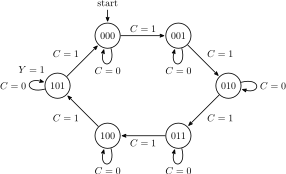
\includegraphics[width=250.3pt]{lect_8_modulo_6_counter}\caption{state diagram}
\end{subfigure}
\caption{Modulo-6 counter with enable.}
\end{figure}

\begin{figure}[htbp]
\centering
\ContinuedFloat
\begin{subfigure}[b]{356.9pt}\centering
  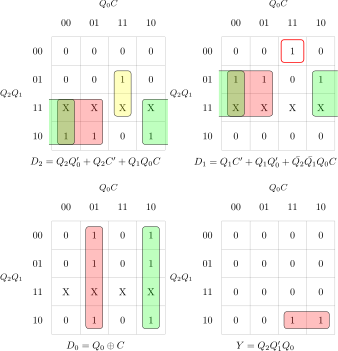
\includegraphics[width=354.9pt]{lect_8_modulo_6_kmaps}\caption{K-maps}\label{fig:mod6-km}
\end{subfigure}
\caption[]{Modulo-6 counter with enable.}
\end{figure}

\begin{figure}[htbp]
\centering
\ContinuedFloat
\begin{subfigure}[b]{412.0pt}\centering
  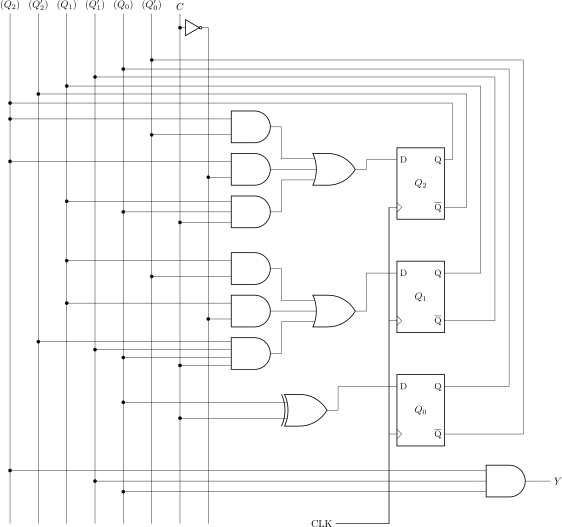
\includegraphics[width=410.0pt]{lect_8_modulo_6_circuit}\caption{logic diagram}\label{fig:mod6-circ}
\end{subfigure}
\caption[]{Modulo-6 counter with enable.}
\end{figure}

\vhdlfile{listings/ch08_modulo6_behav.vhd}{Behavioural VHDL of the modulo-6 counter with enable.}{lst:mod6}

\paragraph{Type conversions in VHDL.} \Cref{lst:mod6} adds one to a vector with the expression
\begin{center}\code{std_logic_vector(unsigned(count) + 1)}\end{center} VHDL is a strongly typed language: arithmetic is defined for the types \code{unsigned} and \code{signed} of the package \code{numeric_std}, not for \code{std_logic_vector}, so one converts explicitly (\cref{fig:conv}). Type-cast functions: \code{unsigned(slv)} and \code{signed(slv)} reinterpret a \code{std_logic_vector}; \code{std_logic_vector(u)} converts back. Integers are converted with \code{to_unsigned(int, size)} and \code{to_signed(int, size)}, and numbers with \code{to_integer(u)} or \code{to_integer(s)}. The conversions of vectors are only reinterpretations of the same bits and cost no hardware.

\figw{410.0pt}{lect_8_vhdl_type_conversion}{Conversions among \code{std_logic_vector}, \code{unsigned}, \code{signed} and \code{integer} in \code{numeric_std}.}{fig:conv}

\subsection{A one-shot circuit}\label{sec:oneshot}
\begin{example}{One-shot}{oneshot}
Design a circuit that produces an output pulse $S=1$ for \emph{exactly one clock cycle} when a push-button input $B$ is pressed, however long the button is held. (Assume the button is already debounced.)

\textbf{Mealy design.} Three states: $S_0$ waits for $B=1$; $S_1$ is the pulse state, always followed by $S_2$ on the next clock; $S_2$ waits for $B=0$ (release) and then returns to $S_0$. Encoding $S_0=00$, $S_1=01$, $S_2=10$, with the unused state 11 returning to 00 (\cref{tab:oneshot}, \cref{fig:os-fsm}), and taking the output as $S=1$ in $S_0$ when $B=1$ (the Mealy output), the K-maps (\cref{fig:os-km}) give
\[
 D_1 = Q_1'Q_0 + Q_1Q_0'B,\qquad D_0 = Q_1'Q_0'B,\qquad S = Q_1'Q_0'B .
\]
The circuit is \cref{fig:os-circ}, the response to a long press is \cref{fig:os-timing}, and \cref{lst:os-mealy} the VHDL.
\end{example}

\begin{table}[htbp]
\centering
\caption{State table of the Mealy one-shot.}
\label{tab:oneshot}
\begin{tabular}{l|c|c|c}
\toprule PS $(Q_1Q_0)$ & NS ($B=0$) & NS ($B=1$) & $S$ (with $B=1$)\\ \midrule
$S_0$ (00)&00&01&1\\ $S_1$ (01)&10&10&0\\ $S_2$ (10)&00&10&0\\ unused (11)&00&00&0\\ \bottomrule
\end{tabular}
\end{table}

\begin{sidewaysfigure}[htbp]
\centering
\begin{subfigure}[b]{244.7pt}\centering
  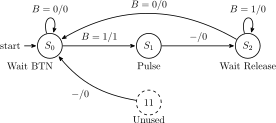
\includegraphics[width=242.7pt]{lect_8_one_shot_fsm}\caption{state diagram}\label{fig:os-fsm}
\end{subfigure}
\caption{The Mealy one-shot circuit.}
\end{sidewaysfigure}

\begin{sidewaysfigure}[htbp]
\centering
\ContinuedFloat
\begin{subfigure}[b]{499.7pt}\centering
  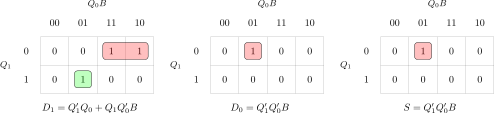
\includegraphics[width=497.7pt]{lect_8_one_shot_kmaps}\caption{K-maps}\label{fig:os-km}
\end{subfigure}
\caption[]{The Mealy one-shot circuit.}
\end{sidewaysfigure}

\begin{sidewaysfigure}[htbp]
\centering
\ContinuedFloat
\begin{subfigure}[b]{313.1pt}\centering
  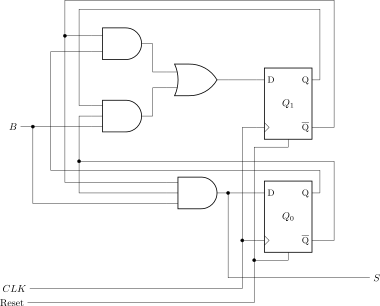
\includegraphics[width=311.1pt]{lect_8_one_shot_circuit}\caption{logic diagram}\label{fig:os-circ}
\end{subfigure}
\caption[]{The Mealy one-shot circuit.}
\end{sidewaysfigure}

\begin{sidewaysfigure}[htbp]
\centering
\ContinuedFloat
\begin{subfigure}[b]{463.4pt}\centering
  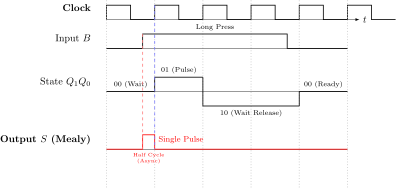
\includegraphics[width=461.4pt]{lect_8_one_shot_timing}\caption{response to a long press}\label{fig:os-timing}
\end{subfigure}
\caption[]{The Mealy one-shot circuit.}
\end{sidewaysfigure}

\vhdlfile{listings/ch08_oneshot_mealy.vhd}{VHDL of the Mealy one-shot.}{lst:os-mealy}

\paragraph{A problem with the Mealy design.} Because $S=Q_1'Q_0'B$ depends directly on the input $B$, which is not synchronised with the clock, the pulse starts when the button is pressed and ends at the next clock edge; its width is therefore \emph{less than one clock period} and varies with the moment of pressing (and any noise on $B$ passes straight to $S$). A \textbf{Moore} design solves the problem: the machine has states $S_0$ (idle, output 0, wait for $B=1$), $S_1$ (pulse, output 1, unconditionally to $S_2$) and $S_2$ (wait for $B=0$), and the output $S=1$ only in the state $S_1$. Since states change only at clock edges, the pulse starts and ends at clock edges and lasts \emph{exactly one period} (\cref{fig:os-moore,fig:os-comp}, \cref{lst:os-moore}). The price is a delay of one clock period between the press and the pulse.

\begin{figure}[htbp]
\centering
\begin{subfigure}[b]{182.9pt}\centering
  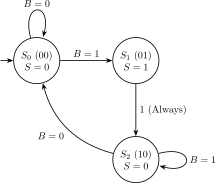
\includegraphics[width=180.9pt]{lect_8_one_shot_moore_fsm}\caption{Moore state diagram}\label{fig:os-moore}
\end{subfigure}
\\[6pt]
\begin{subfigure}[b]{412.0pt}\centering
  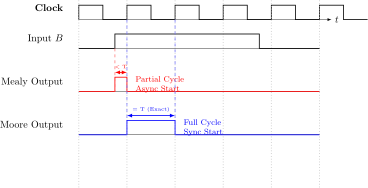
\includegraphics[width=410.0pt]{lect_8_one_shot_comparison}\caption{Mealy (asynchronous) and Moore (synchronous) pulse}\label{fig:os-comp}
\end{subfigure}
\caption{The Moore one-shot and the comparison of the two outputs.}
\end{figure}

\vhdlfile{listings/ch08_oneshot_moore.vhd}{VHDL of the Moore one-shot (exact one-cycle pulse).}{lst:os-moore}

\paragraph{VHDL coding of Moore and Mealy machines.} The two styles differ in a recognisable way, summarised in \cref{tab:vhdl-style}. In a Moore machine the outputs are assigned depending on \code{current_state} only; in a Mealy machine the output assignments are inside the \code{if} statements that test the inputs, so the process must be sensitive to the inputs as well.

\begin{table}[htbp]
\centering
\small
\caption{VHDL coding differences between Moore and Mealy machines.}
\label{tab:vhdl-style}
\begin{tabularx}{\linewidth}{@{}lXX@{}}
\toprule
 & \textbf{Moore} & \textbf{Mealy}\\ \midrule
Sensitivity list & \code{process(current_state)} (and the inputs for the next-state logic) & \code{process(current_state, inputs)}\\
Output assignment & outside any test of inputs within the \code{case} branch: \code{when S0 => A <= '1'; next_state <= S1;} & inside \code{if}/\code{case} tests of inputs: \code{when S0 => if X='1' then A<='1'; else A<='0'; end if;}\\
Timing & output stable between clock edges (comes from the state register) & output may change whenever an input changes\\ \bottomrule
\end{tabularx}
\end{table}

\subsection{A control unit}
\begin{example}{A simple processor control unit}{cpu}
An FSM is also the form of the \emph{control unit} of a processor (\cref{ch:dedicated}): it steps through the actions of a computation in response to status signals. The machine in \cref{fig:cpu-fsm} has states $s_0,\dots,s_3$ and outputs $x$ and $y$; the transitions out of $s_0$ depend on the input \textit{Start} ($Start$ and $Start'$), and those out of $s_2$ on the status signal $n=9$ ($n=9$ and $(n=9)'$). The remaining transitions are unconditional. Such a machine is synthesised exactly as the others in this chapter; note that its inputs are \emph{comparisons} produced by other circuits, a feature that we exploit in \cref{ch:dedicated,ch:gp}.
\end{example}

\figw{234.5pt}{lect_8_simple_cpu_fsm_example}{State diagram of the control unit of \cref{ex:cpu}.}{fig:cpu-fsm}

\subsection{An elevator controller: Moore and Mealy}
\begin{example}{Two-floor elevator controller (Moore)}{elev-moore}
Design the FSM for an elevator serving two floors (\cref{fig:elev-setup}). Inputs: $f_1,f_2$ are the call buttons for floors 1 and 2 (hall and cabin buttons combined, assumed to stay pressed until served) and $at_1,at_2$ are position sensors, asserted when the cabin is at floor 1 or 2. Outputs: $go_1$ (motor on) and $go_0$ (direction, $0$ = down, $1$ = up), and the floor indicators $led_1$ and $led_2$.

\textbf{State diagram} (\cref{fig:elev-moore}). Four states: \textbf{00} floor 1 (idle; $led_1$ on; on $f_2$ go to 11); \textbf{11} moving up ($go_1=go_0=1$; on $at_2$ go to 10); \textbf{10} floor 2 (idle; $led_2$ on; on $f_1$ go to 01); \textbf{01} moving down ($go_1=1,go_0=0$; on $at_1$ go to 00). The motor outputs depend on the state only, so this is a Moore machine.

\textbf{Equations.} From the K-maps of \cref{fig:elev-moore-km},
\begin{align*}
 D_1 &= Q_1'Q_0'f_2 + Q_1Q_0 + Q_1Q_0'f_1',\\
 D_0 &= Q_1'Q_0'f_2 + Q_1Q_0\,at_2' + Q_1Q_0'f_1 + Q_1'Q_0\,at_1' .
\end{align*}
Each term describes one transition: for example $Q_1Q_0\,at_2'$ keeps $D_0=1$ while the cabin moves up and has not yet arrived. \Cref{lst:elev-moore} is the VHDL.
\end{example}

\begin{figure}[htbp]
\centering
\begin{subfigure}[b]{338.4pt}\centering
  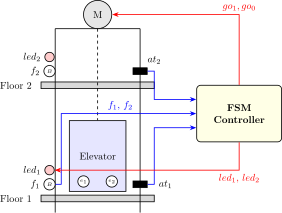
\includegraphics[width=336.4pt]{lect_8_elevator_setup}\caption{system}\label{fig:elev-setup}
\end{subfigure}
\caption{Two-floor elevator controller, Moore version.}
\end{figure}

\begin{figure}[htbp]
\centering
\ContinuedFloat
\begin{subfigure}[b]{282.0pt}\centering
  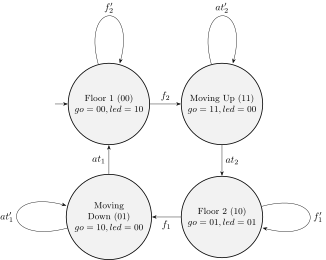
\includegraphics[width=280.0pt]{lect_8_elevator_fsm}\caption{Moore state diagram}\label{fig:elev-moore}
\end{subfigure}
\\[6pt]
\begin{subfigure}[b]{252.3pt}\centering
  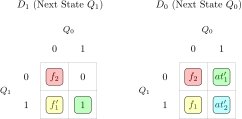
\includegraphics[width=250.3pt]{lect_8_elevator_moore_kmaps}\caption{K-maps for $D_1$, $D_0$}\label{fig:elev-moore-km}
\end{subfigure}
\caption[]{Two-floor elevator controller, Moore version.}
\end{figure}

\vhdlfile{listings/ch08_elevator_moore.vhd}{VHDL of the Moore elevator controller (four states).}{lst:elev-moore}

\begin{example}{Two-floor elevator controller (Mealy)}{elev-mealy}
The same controller can be built with only \emph{two} states, \textit{Floor1} and \textit{Floor2}, if the motor outputs are allowed to depend on the buttons. The state changes only when the cabin \emph{arrives} at a floor ($at_x$); the motor is turned on by the call button of the \emph{other} floor (\cref{fig:elev-mealy}):
\begin{align*}
 D &= \NOT{Q}\,(f_2\cdot at_2) + Q\,\overline{(f_1\cdot at_1)},\\
 led_1 &= \NOT{Q},\quad led_2 = Q,\quad go_1 = \NOT{Q}f_2 + Qf_1,\quad go_0 = \NOT{Q}.
\end{align*}
With $Q=0$ (floor 1) and $f_2$ pressed the motor runs upwards until $at_2$ arrives; the K-maps are \cref{fig:elev-mealy-km} and the VHDL \cref{lst:elev-mealy}. The state memory shrinks from two flip-flops to one, but the output logic becomes more complex, and the outputs now respond directly to the buttons. In this version the indicators show the last floor served, not the cabin position while it moves.
\end{example}

\begin{figure}[htbp]
\centering
\begin{subfigure}[b]{202.1pt}\centering
  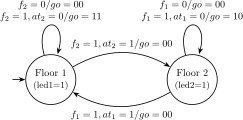
\includegraphics[width=200.1pt]{lect_8_elevator_mealy_fsm}\caption{Mealy state diagram}\label{fig:elev-mealy}
\end{subfigure}
\\[6pt]
\begin{subfigure}[b]{228.7pt}\centering
  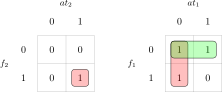
\includegraphics[width=226.7pt]{lect_8_elevator_mealy_kmaps}\caption{K-maps}\label{fig:elev-mealy-km}
\end{subfigure}
\caption{Two-floor elevator controller, Mealy version.}
\end{figure}

\vhdlfile{listings/ch08_elevator_mealy.vhd}{VHDL of the Mealy elevator controller (two states).}{lst:elev-mealy}

\section{Moore versus Mealy Timing}\label{sec:moore-mealy}
The essential difference is the timing of the outputs (\cref{fig:mm-timing}). A Moore output changes only just after a clock edge, because it is a function of the state register, so it is synchronous and stable for the whole period. A Mealy output can change at any time during the period when an input changes: it \emph{reacts one clock period earlier} than the equivalent Moore output, but it can also show glitches if the inputs change at different times, and in a chain of Mealy machines such combinational paths from input to output add up. The elevator timing diagram, \cref{fig:elev-timing}, shows a complete trip with the two versions.

\begin{sidewaysfigure}[htbp]
\centering
\begin{subfigure}[b]{544.8pt}\centering
  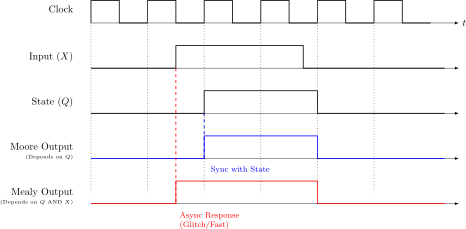
\includegraphics[width=542.8pt]{lect_8_moore_vs_mealy_timing}\caption{generic timing comparison}\label{fig:mm-timing}
\end{subfigure}
\caption{Moore and Mealy output timing.}
\end{sidewaysfigure}

\begin{sidewaysfigure}[htbp]
\centering
\ContinuedFloat
\begin{subfigure}[b]{602.0pt}\centering
  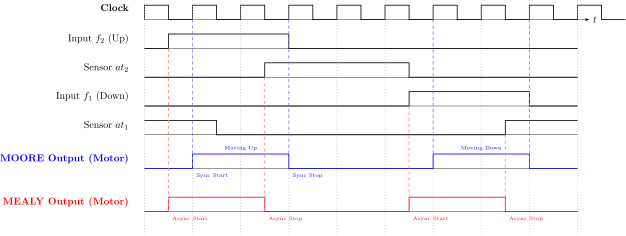
\includegraphics[width=600.0pt]{lect_8_elevator_timing}\caption{elevator, up and down}\label{fig:elev-timing}
\end{subfigure}
\caption[]{Moore and Mealy output timing.}
\end{sidewaysfigure}

\begin{keypoint}[Choosing between Moore and Mealy]
Use a \textbf{Moore} machine when the outputs must be glitch-free and aligned with the clock, or drive other synchronous logic (the usual choice). Use a \textbf{Mealy} machine when you need the fastest reaction or the smallest number of states, and take care that the inputs are synchronised. Any Mealy machine has an equivalent Moore machine, usually with more states.
\end{keypoint}

\section{Timing of a Synchronous FSM}\label{sec:fsm-timing}
All state changes occur at the active clock edge, but the next state must be \emph{ready} before the next edge. The signal path is: clock edge $\to$ flip-flop output ($t_{pcq}$, the propagation delay from clock to $Q$) $\to$ next-state logic ($t_{comb}$) $\to$ flip-flop input, which must be stable for the \emph{setup time} $t_{setup}$ before the next edge. Hence
\begin{equation}
  T_{clk} \;\ge\; t_{pcq} + t_{comb} + t_{setup},\qquad f_{max}=\frac{1}{t_{pcq}+t_{comb}+t_{setup}} .
  \label{eq:fmax}
\end{equation}
If $t_{pcq}=0.5$~ns, $t_{comb}=3$~ns and $t_{setup}=0.2$~ns, then $T_{clk}\ge3.7$~ns and $f_{max}\approx270$~MHz. In addition the inputs must remain stable for the \emph{hold time} $t_{hold}$ after the edge. Equation~\eqref{eq:fmax} explains why a design with more complex next-state logic (a longer $t_{comb}$) must run slower, and why one-hot encoding, with its simpler logic, is often faster.

\section{A Template for VHDL State Machines}
Most FSMs in this book follow one template.

\begin{lstlisting}[caption={Template of the two-process FSM description (the state register is process 1 and the combinational logic process 2).},label={lst:fsm-template}]
architecture fsm of my_machine is
  type state_type is (S0, S1, S2);                  -- list the states
  signal current_state, next_state : state_type;
begin
  -- Process 1: state register (sequential)
  process (clk, reset)
  begin
    if reset = '1' then
      current_state <= S0;                          -- initial state
    elsif rising_edge(clk) then
      current_state <= next_state;
    end if;
  end process;

  -- Process 2: next-state and output logic (combinational)
  process (current_state, x)                        -- all signals that are read
  begin
    next_state <= current_state;                    -- defaults: stay, outputs inactive
    y <= '0';
    case current_state is
      when S0 => if x = '1' then next_state <= S1; end if;
      when S1 => y <= '1'; next_state <= S2;        -- Moore output
      when S2 => if x = '0' then next_state <= S0; end if;
    end case;
  end process;
end fsm;
\end{lstlisting}

A common error is to omit a signal from the sensitivity list: for example, writing \code{process(clk)} for the register above without \code{reset} makes the asynchronous reset ineffective in simulation. In process 2 the sensitivity list must contain \emph{every signal that is read}.

\begin{chaptersummary}
\begin{itemize}
  \item An \textbf{FSM} has next-state logic, a state register and output logic. \textbf{Moore}: output = $f$(state). \textbf{Mealy}: output = $f$(state, inputs).
  \item \textbf{Analysis}: equations $\to$ state table $\to$ state diagram. \textbf{Synthesis}: specification $\to$ state diagram $\to$ state table $\to$ (minimisation) $\to$ state assignment $\to$ flip-flop type $\to$ K-maps $\to$ logic diagram or VHDL.
  \item \textbf{State encodings}: binary (fewest flip-flops), Gray, one-hot ($N$ flip-flops, simpler logic).
  \item In VHDL use an \textbf{enumerated state type} and the \textbf{two-process method}; assign defaults to avoid latches; use \code{numeric_std} and explicit conversions for arithmetic.
  \item The \textbf{one-shot} shows the difference between the models: the Mealy output is asynchronous (less than one clock), the Moore output is exactly one cycle but delayed.
  \item The clock period must satisfy $T_{clk}\ge t_{pcq}+t_{comb}+t_{setup}$.
\end{itemize}
\end{chaptersummary}

\chapsec{Exercises}
\begin{exlist}
  \item \textbf{Moore or Mealy?} Machine (A) has next-state logic with inputs \{inputs, present state\} and output logic with inputs \{present state\}. Machine (B) has output logic with inputs \{inputs, present state\}. Which is Moore and which is Mealy?
  \item \textbf{State analysis.} A state machine has one JK flip-flop with $J=x$ and $K=1$. If the present state is $Q=0$ and $x=1$, what is the next state? Give the complete state table.
  \item \textbf{110 detector, overlapping.} Draw the state diagram of a Mealy sequence detector for the sequence \texttt{110} in which overlapping sequences are valid. For the input \texttt{0 1 1 0 1 1 0} the output must be \texttt{0 0 0 1 0 0 1}.
  \item \textbf{110 detector, non-overlapping.} Draw the state diagram of a \emph{non-overlapping} detector for \texttt{110}: after a detection the machine returns to the initial state. Explain why the two diagrams are the same for the sequence \texttt{110} but would differ for \texttt{101}.
  \item \textbf{State encoding.} An FSM has 12 states. How many flip-flops are needed with (a)~binary encoding; (b)~one-hot encoding?
  \item \textbf{VHDL syntax.} What is missing in the sensitivity list of this synchronous-FSM state-register process? \begin{lstlisting}
process (clk)
begin
  if reset = '1' then current_state <= S0;
  elsif rising_edge(clk) then current_state <= next_state;
  end if;
end process;
\end{lstlisting}
  \item \textbf{State-table construction.} Counter sequence $00\to01\to10\to11\to00$ with an input that is 0 for hold and 1 for count. Give the missing next state for present state $01$ and input 1.
  \item \textbf{Logic equation.} In the K-map of \cref{fig:ex88} for $D_0$ (rows $Q$, columns $X$), derive the simplified Boolean equation.
  \item \textbf{Timing.} Which of the following correctly bounds the clock period of an FSM? (1)~$T_{clk}\ge t_{setup}+t_{hold}$; (2)~$T_{clk}\ge t_{pcq}+t_{comb}+t_{setup}$; (3)~$T_{clk}\ge t_{pcq}+t_{comb}-t_{hold}$. Compute $f_{max}$ if $t_{pcq}=0.4$~ns, $t_{comb}=2.1$~ns and $t_{setup}=0.3$~ns.
  \item \textbf{Gray-code counter.} Design a 2-bit Gray-code counter with the sequence $00\to01\to11\to10\to00$: draw the state diagram, find the D flip-flop equations and the circuit.
  \item Convert the Mealy 101 detector of \cref{ex:seqdet} to a \emph{Moore} machine. How many states are needed? Draw the state diagram.
  \item Design a Moore FSM for a simple traffic light with states Green, Yellow and Red, which changes state on every clock pulse when an input \code{tick} is 1. Give the state diagram, a binary state assignment, the equations and VHDL.
  \item Write the VHDL of a Moore machine whose output $z$ is 1 while the input $x$ has been 1 for at least three consecutive clock cycles.
  \item Explain, with a sketch, why the output of a Mealy machine can show a glitch when two inputs change at slightly different times, and why a Moore output cannot.
  \item For the Mealy one-shot, draw the waveforms of $B$, the clock and $S$ if $B$ rises between two clock edges and falls after three clock periods. Compare with the Moore version.
\end{exlist}

\begin{figure}[htbp]
\centering
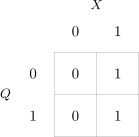
\includegraphics[width=129pt]{lect_8_exercise_8_8_kmap}
\caption{K-map for Exercise~8.8.}
\label{fig:ex88}
\end{figure}

\chapsec{Further Reading}
Mealy's and Moore's original papers~\cite{mealy1955,moore1956} introduced the two models. The synthesis of FSMs and their VHDL descriptions are treated in Chapter~8 of Brown and Vranesic~\cite{brown2009} and Chapter~5 of Hwang~\cite{hwang2005}; the coding templates for state machines follow Ashenden~\cite{ashenden2008}. Gajski~\cite{gajski1997} extends FSMs with a datapath, the topic of the next chapter.
